\documentclass[tikz]{standalone}
\usepackage{tikz}
    \usetikzlibrary{positioning}

\tikzset{basic/.style={draw,fill=cyan!20,text width=1em,text badly centered}}
\tikzset{input/.style={fill=red!40,circle}}
\tikzset{weights/.style={basic,circle}}
\tikzset{functions/.style={basic,circle,fill=cyan!40}}
\tikzset{output/.style={basic,circle,fill=blue!60!green!45}}

\begin{document}
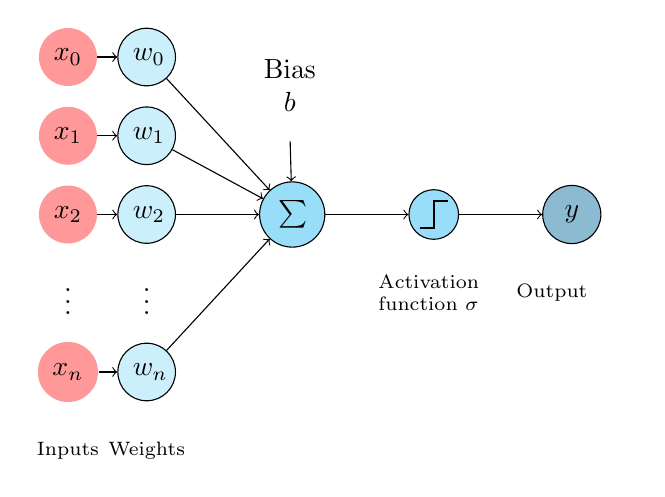
\begin{tikzpicture}
%    \node[functions] (center){output}
 
    \node[functions] (center) {};  
    \node[output, right=3em of center] (right) {$y$};
       \path[draw,->] (center)--(right);
    \node[below of=right,font=\scriptsize,text width=4em] {Output};
 
    \node[below of=center,font=\scriptsize,text width=4em] {Activation function $\sigma$};
    
   \draw[thick] (0.5em,0.5em) -- (0,0.5em) -- (0,-0.5em) -- (-0.5em,-0.5em);
%    \draw (0em,0.75em) -- (0em,-0.75em);
%    \draw (0.75em,0em) -- (-0.75em,0em);

    \node[functions,left=3em of center] (left) {$\sum$};
        \path[draw,->] (left) -- (center);
        
    \node[label=above:\parbox{1cm}{\centering Bias \\ $b$}] at (-5.2em, 3.0em) (b) {}; 
        \path[draw,->] (b) -- (left);
    \node[weights,left=3em of left] (2) {$w_2$} -- (2) node[input,left of=2] (l2) {$x_2$};
        \path[draw,->] (l2) -- (2);
        \path[draw,->] (2) -- (left);   


    
    \node[below of=2] (dots) {$\vdots$} -- (dots) node[left of=dots] (ldots) {$\vdots$};
    \node[weights,below of=dots] (n) {$w_n$} -- (n) node[input,left of=n] (ln) {$x_n$};
        \path[draw,->] (ln) -- (n);
        \path[draw,->] (n) -- (left);
        
    \node[weights,above of=2] (1) {$w_1$} -- (1) node[input,left of=1] (l1) {$x_1$};
        \path[draw,->] (l1) -- (1);
        \path[draw,->] (1) -- (left);
        
    \node[weights,above of=1] (0) {$w_0$} -- (0) node[input,left of=0] (l0) {$x_{0}$};
        \path[draw,->] (l0) -- (0);
        \path[draw,->] (0) -- (left);
        
    \node[below of=ln,font=\scriptsize] {Inputs};
    \node[below of=n,font=\scriptsize] {Weights};
\end{tikzpicture}
\end{document}